%!TEX root=paper.tex
\section{Method}\label{sec:method}

Our method builds on the architecture described in \cite{Girshick-CVPR-2014}.
As summarized in \autoref{fig:rcnn}, R-CNN starts with external region-of-interest proposals (ROIs), and then does the following: (1) for each ROI, classifies it with a CNN, obtaining multi-class scores; (2) post-processes the scored ROIs with non-maximal suppression and other bounding box refinement to obtain the final detections.

We aim to incorporate several speed-ups into a similar architecture.
As summarized in \autoref{fig:combined}, we start with the same ROI proposals, and then (1) score each proposal with a quick-to-compute feature; (2) select the ROI that is most promising, and score it with a CNN, which is additionally sped up with a cascaded structure; (3a) either select another ROI, incorporating the scores of the first one into the selection -- or (3b) post-process the ROIs scored so far and exit.

For the quick feature, we consider the CNN pixel gradient in \autoref{sec:gradient} and an amortized R-CNN variant that operates on a feature pyramid in \autoref{sec:dense}.
The Cascaded CNN is described in \autoref{sec:ccnn}.
The dynamic region selection is explained in \autoref{sec:dynamic}.

\begin{figure}[h!]
\begin{center}
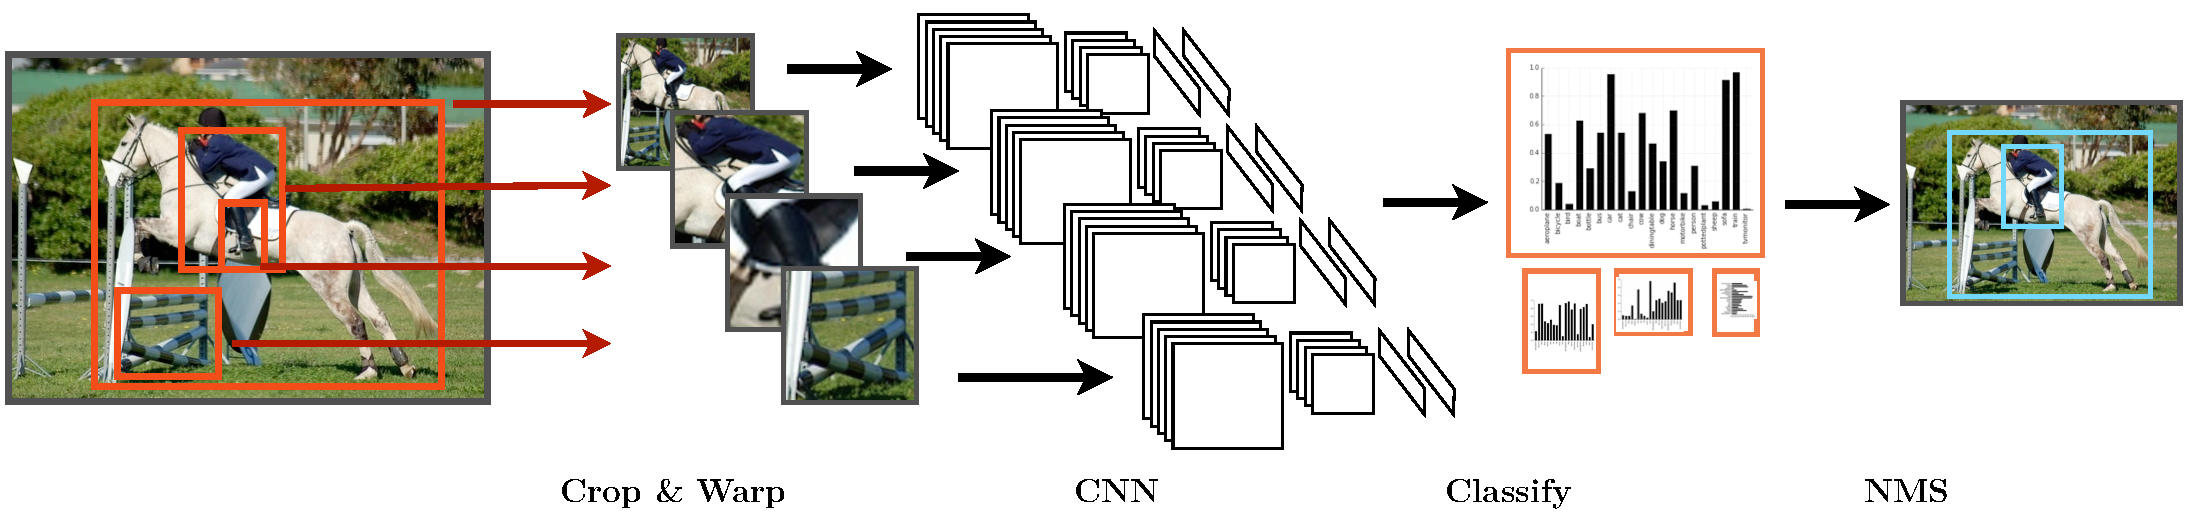
\includegraphics[width=0.98\columnwidth]{figures/rcnn.pdf}
\caption{
R-CNN architecture: image regions are cropped, resized, and each one fed through a CNN with classification layers.
The classifier outputs are post-processed to give the final detections.
}\label{fig:rcnn}
\end{center}
\end{figure}

\begin{figure}[h!]
\begin{center}
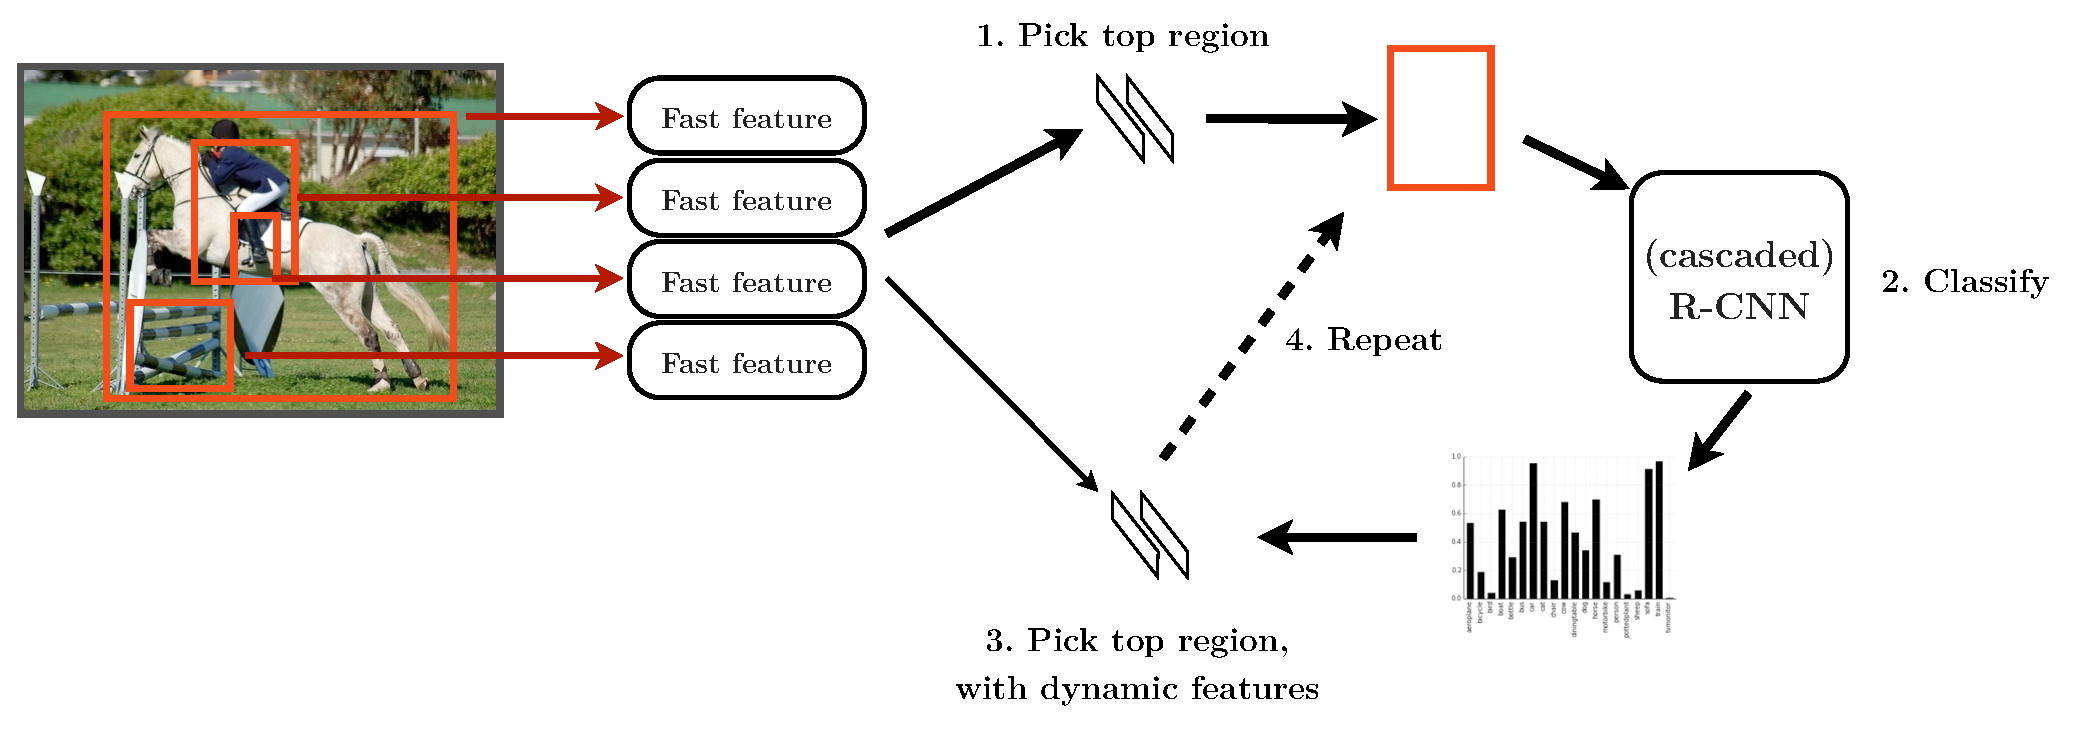
\includegraphics[width=0.98\columnwidth]{figures/combined.pdf}
\caption{
Dynamic region selection combines both speedups and introduces another.
}\label{fig:combined}
\end{center}
\end{figure}

%%%%%%%%%%%%%%%%%%%%%%%%%%%%%%%%%%%%%%%%%%%%%%%%%%%%%%%%%%%%%%%%%%%%%%%%%%%%%%%
\subsection{CNN pixel gradient computation}\label{sec:gradient}

One fast-to-compute feature we consider for the preliminary featurization of ROIs is the pixel gradient, back-propagated throgh the classifier CNN applied to the whole image.
This gradient corresponds to a kind of saliency map onto the image \cite{Simonyan-ICLR-2014}, and can therefore be used to evaluate ROIs.

\begin{itemize}
\itemsep1pt\parskip0pt\parsep0pt
\item
    \todo{Explain backprop to pixels.}
\item
    \todo{Explain how we featurize it: warp each ROI to canonical size and also include overall statistics, then train to classify $>0.3$ overlap with ground truth.}
\item
    \todo{FIGURE: shows schematic structure of the flow and gradient saliency maps for a couple of images.}
\end{itemize}

\lorem{Lorem ipsum dolor sit amet, consectetur adipisicing elit, sed do eiusmod tempor incididunt ut labore et dolore magna aliqua. Ut enim ad minim veniam, quis nostrud exercitation ullamco laboris nisi ut aliquip ex ea commodo consequat. Duis aute irure dolor in reprehenderit in voluptate velit esse cillum dolore eu fugiat nulla pariatur. Excepteur sint occaecat cupidatat non proident, sunt in culpa qui officia deserunt mollit anim id est laborum.}

%%%%%%%%%%%%%%%%%%%%%%%%%%%%%%%%%%%%%%%%%%%%%%%%%%%%%%%%%%%%%%%%%%%%%%%%%%%%%%%
\subsection{Pyramid amortized R-CNN}\label{sec:dense}

Another fast ROI featurization we consider is a variant of R-CNN that processes the whole image, at multiple scales, with the CNN up to the topmost non-fully-connected layer.
We call this multiscale CNN output a ``feature pyramid''.
As \autoref{fig:dense_rcnn} shows, ROIs are then cropped from the feature pyramid at the best matching scale, warped to a canonical size, and classified.
ROIs are highly overlapping, but their featurization is shared through the pyramid, amortizing its construction cost.
This doesn't work as well as the original R-CNN system, but is much faster, and can therefore be used as the fast feature for the dynamic region selection.

\subsubsection{Design choices}

We explored a variety of choices while designing Pyramid R-CNN.
We tried using a single scale or a pyramid with 7 levels each separated by a scale factor of $2^{-1/2}$.
For warping, we experimented with canonical sizes of $s \times s$, for $s \in \{5,6,7\}$ and resampling with nearest neighbor or bilinear interpolation.
We also tried two variants of the feature pyramid: the raw feature pyramid or one where each level is max pooled with a $3 \times 3$ pooling window run at a stride of $1$ (to avoid subsampling).

Table ??? shows mAP performance on PASCAL VOC 2007 test for these various choices.
The best configuration, in terms of mAP, uses a 7 level pyramid, a warp size of $7 \times 7$ with bilinear interpolation, and max pooling.
The first level of our pyramid is computed from a $1713 \times 1713$ pixel image, which yields a $108 \times 108$ cell feature map.
The gold standard (non-pyramid) R-CNN performance using the same non-fine-tuned CNN is 44.2\% mAP.
Our best result with Pyramid R-CNN is slightly worse, at 41.9\%.

To map a ROI $R$ into the pyramid, we start by computing an ``optimal'' scale defined by $\alpha^* = 227/\min(h,w)$, where $h$ and $w$ are image height and width of $R$.
We then find the nearest level in the pyramid: $l^* = \textrm{argmin}_l |\log(\alpha_l) - \log(\alpha^*)|$, where $\alpha_l$ is the scale factor for pyramid level $l$.
This procedure approximates the scale that R-CNN would use, since it operates on $227$ pixel inputs.


\begin{itemize}
\itemsep1pt\parskip0pt\parsep0pt
\item
  %\todo{Explain design choices (single vs multi scale, finding nearest window, warping.}
  \todo{Add table}
\end{itemize}

%\lorem{Lorem ipsum dolor sit amet, consectetur adipisicing elit, sed do eiusmod tempor incididunt ut labore et dolore magna aliqua. Ut enim ad minim veniam, quis nostrud exercitation ullamco laboris nisi ut aliquip ex ea commodo consequat. Duis aute irure dolor in reprehenderit in voluptate velit esse cillum dolore eu fugiat nulla pariatur. Excepteur sint occaecat cupidatat non proident, sunt in culpa qui officia deserunt mollit anim id est laborum.}

\begin{figure}[h!]
\begin{center}
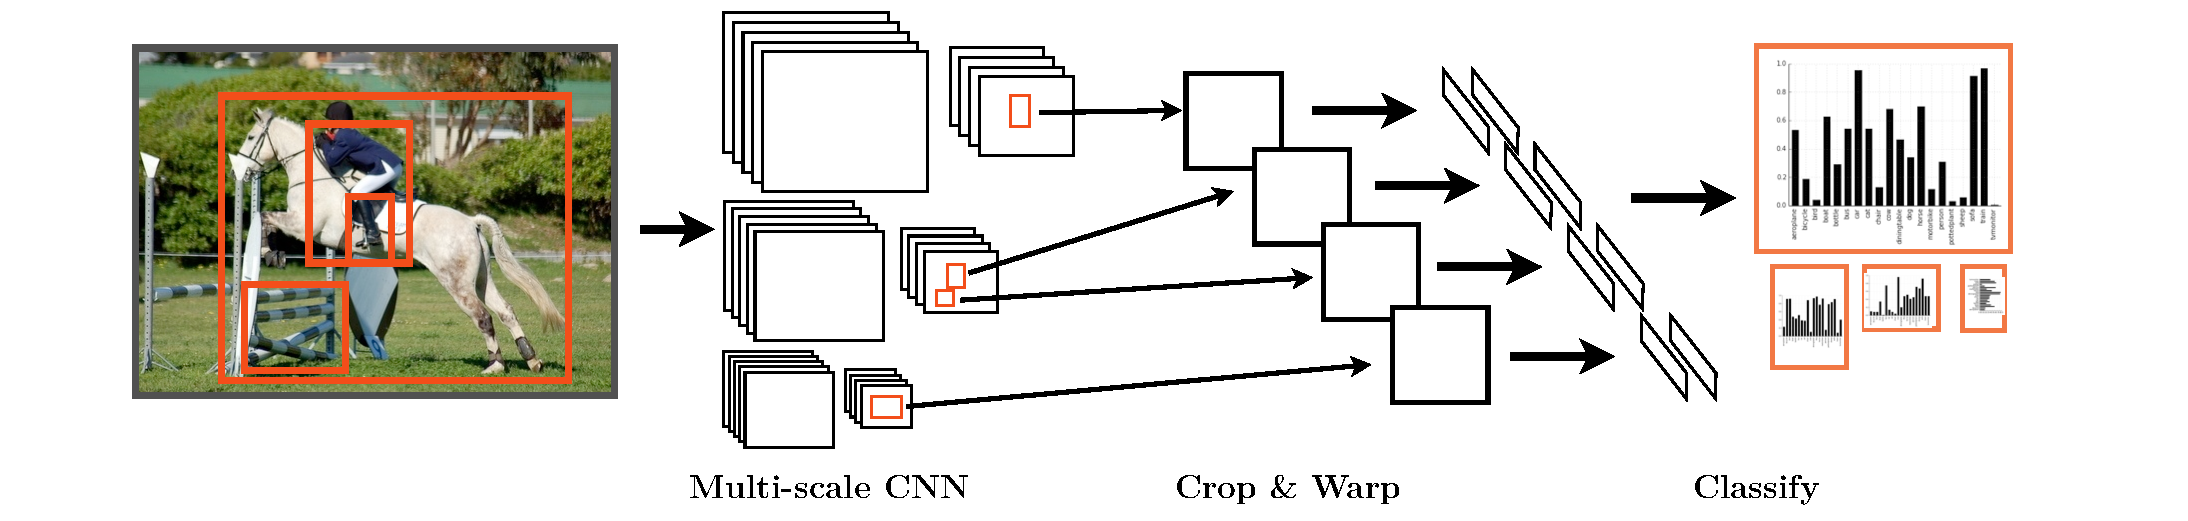
\includegraphics[width=0.98\columnwidth]{figures/dense_rcnn.pdf}
\caption{
Post R-CNN architecture: the whole image is fed through a CNN up to the highest pooling layer.
Regions are cropped from that layer at the best matching scale, resized, and classified.
}\label{fig:dense_rcnn}
\end{center}
\end{figure}

%%%%%%%%%%%%%%%%%%%%%%%%%%%%%%%%%%%%%%%%%%%%%%%%%%%%%%%%%%%%%%%%%%%%%%%%%%%%%%%
\subsection{Cascaded CNN}\label{sec:ccnn}

Most ROIs that go through the CNN in R-CNN do not contain objects of interest, and are simply background.
It would be useful to quickly reject these regions, without expending the full amount of computation on them.

The Cascaded CNN, shown in \autoref{fig:ccnn}, augments the CNN network with an ``Early Terminate'' option: after some layers, the network decides whether to keep computing the input with the next layer, or to terminate with a classification.
For our purpose, the terminate layers are trained to separate Background/Foreground, terminating if they are confident that the input is Background.
Only the last classification layer output the full multi-class scores.

\begin{itemize}
\itemsep1pt\parskip0pt\parsep0pt
\item
  \todo{Explain training the thresholds.}
\end{itemize}

\lorem{Lorem ipsum dolor sit amet, consectetur adipisicing elit, sed do eiusmod tempor incididunt ut labore et dolore magna aliqua. Ut enim ad minim veniam, quis nostrud exercitation ullamco laboris nisi ut aliquip ex ea commodo consequat. Duis aute irure dolor in reprehenderit in voluptate velit esse cillum dolore eu fugiat nulla pariatur. Excepteur sint occaecat cupidatat non proident, sunt in culpa qui officia deserunt mollit anim id est laborum.}

\begin{figure}[h!]
\begin{center}
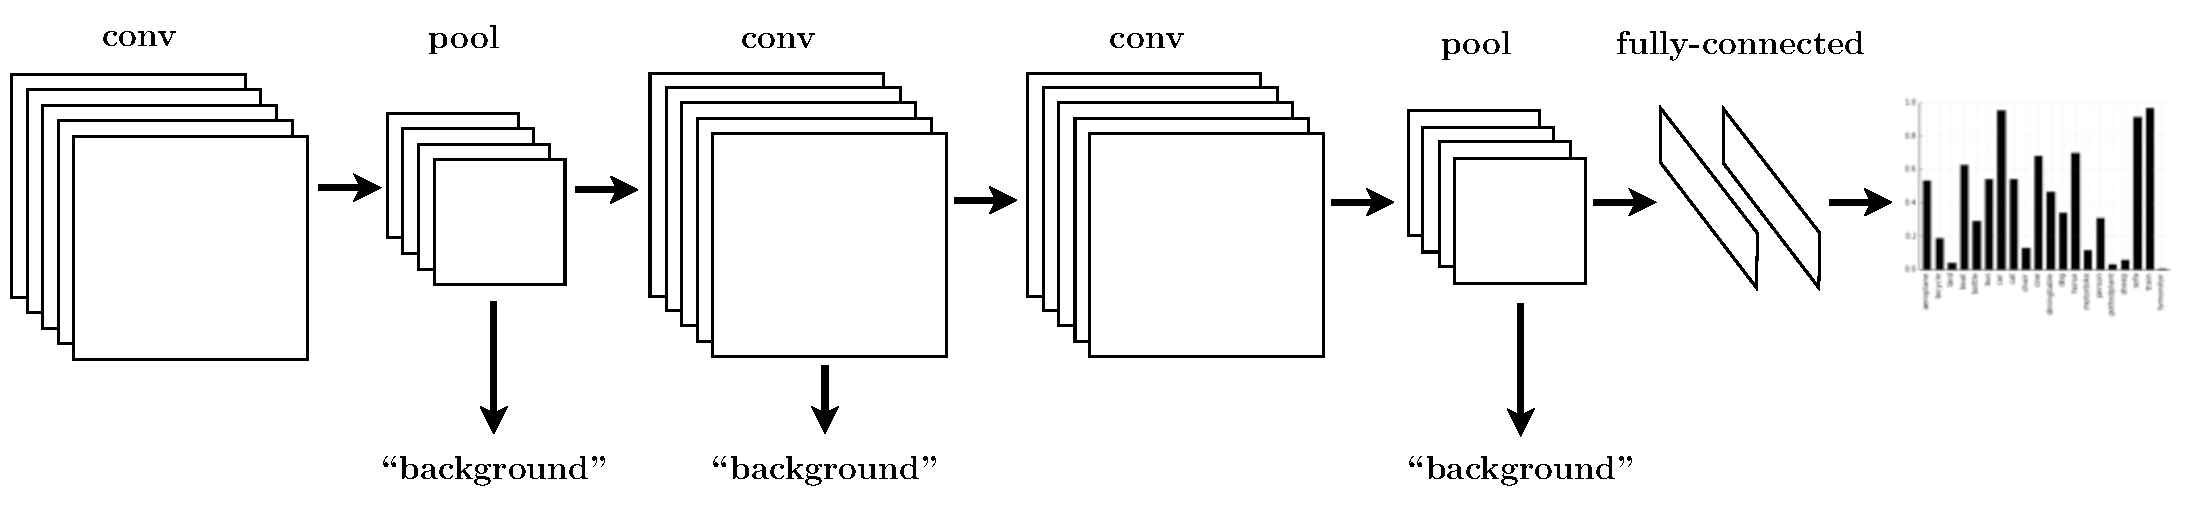
\includegraphics[width=0.98\columnwidth]{figures/ccnn.pdf}
\caption{
The Cascaded CNN has a reject option after certain layers.
\todo{Redo figure to introduce the Reject layers and color their arrows red to make it clear that a choice is being made.}
}\label{fig:ccnn}
\end{center}
\end{figure}

%%%%%%%%%%%%%%%%%%%%%%%%%%%%%%%%%%%%%%%%%%%%%%%%%%%%%%%%%%%%%%%%%%%%%%%%%%%%%%%
\subsection{Dynamic region selection}\label{sec:dynamic}

\autoref{fig:combined} shows the dynamic region selection loop.

\begin{itemize}
\itemsep1pt\parskip0pt\parsep0pt
\item
  \todo{Explain dynamic selection of region batches.}
\item
  \todo{Explain iterative training procedure.}
\end{itemize}

\lorem{Lorem ipsum dolor sit amet, consectetur adipisicing elit, sed do eiusmod tempor incididunt ut labore et dolore magna aliqua. Ut enim ad minim veniam, quis nostrud exercitation ullamco laboris nisi ut aliquip ex ea commodo consequat. Duis aute irure dolor in reprehenderit in voluptate velit esse cillum dolore eu fugiat nulla pariatur. Excepteur sint occaecat cupidatat non proident, sunt in culpa qui officia deserunt mollit anim id est laborum.}

\lorem{Lorem ipsum dolor sit amet, consectetur adipisicing elit, sed do eiusmod tempor incididunt ut labore et dolore magna aliqua. Ut enim ad minim veniam, quis nostrud exercitation ullamco laboris nisi ut aliquip ex ea commodo consequat. Duis aute irure dolor in reprehenderit in voluptate velit esse cillum dolore eu fugiat nulla pariatur. Excepteur sint occaecat cupidatat non proident, sunt in culpa qui officia deserunt mollit anim id est laborum.}
